% ******************************* PhD Thesis Template **************************
% Please have a look at the README.md file for info on how to use the template

\documentclass[a4paper,12pt,times,authoryear,print,index]{Classes/PhDThesisPSnPDFel}

% ******************************************************************************
% ******************************* Class Options ********************************
% *********************** See README for more details ************  **************
% ******************************************************************************

% `a4paper'(The University of Cambridge PhD thesis guidelines recommends a page
% size a4 - default option) or `a5paper': A5 Paper size is also allowed as per
% the Cambridge University Engineering Deparment guidelines for PhD thesis
%
% `11pt' or `12pt'(default): Font Size 10pt is NOT recommended by the University
% guidelines
%
% `oneside' or `twoside'(default): Printing double side (twoside) or single
% side.
%
% `print': Use `print' for print version with appropriate margins and page
% layout. Leaving the options field blank will activate Online version.
%
% `index': For index at the end of the thesis
%
% `draftclassic': For draft mode without loading any images (same as draft in book)
%
% `draft': Special draft mode with line numbers, images, and water mark with
% timestamp and custom text. Position of the text can also be modified.
%
% `abstract': To generate only the title page and abstract page with
% dissertation title and name, to submit to the Student Registry
%
% `chapter`: This option enables only the specified chapter and it's references
%  Useful for review and corrections.
% 
% `extsum`: To print only extended summary in English. Uncomment include file in main
% matter and change language in preample file. 
%
% ************************* Custom Page Margins ********************************
%
% `custommargin`: Use `custommargin' in options to activate custom page margins,
% which can be defined in the preamble.tex. Custom margin will override
% print/online margin setup.
%
% *********************** Choosing the Fonts in Class Options ******************
%
% `times' : Times font with math support. (The Cambridge University guidelines
% recommend using times)
%
% `fourier': Utopia Font with Fourier Math font (Font has to be installed)
%            It's a free font.
%
% `customfont': Use `customfont' option in the document class and load the
% package in the preamble.tex
%
% default or leave empty: `Latin Modern' font will be loaded.
%
% ********************** Choosing the Bibliography style ***********************
%
% `authoryear': For author-year citation eg., Krishna (2013)
%
% `numbered': (Default Option) For numbered and sorted citation e.g., [1,5,2]
%
% `custombib': Define your own bibliography style in the `preamble.tex' file.
%              `\RequirePackage[square, sort, numbers, authoryear]{natbib}'.
%              This can be also used to load biblatex instead of natbib
%              (See Preamble)
%
% **************************** Choosing the Page Style *************************
%
% `default (leave empty)': For Page Numbers in Header (Left Even, Right Odd) and
% Chapter Name in Header (Right Even) and Section Name (Left Odd). Blank Footer.
%
% `PageStyleI': Chapter Name next & Page Number on Even Side (Left Even).
% Section Name & Page Number in Header on Odd Side (Right Odd). Footer is empty.
%
% `PageStyleII': Chapter Name on Even Side (Left Even) in Header. Section Number
% and Section Name in Header on Odd Side (Right Odd). Page numbering in footer


% ********************************** Preamble **********************************
% Preamble: Contains packages and user-defined commands and settings
% ******************************************************************************
% ****************************** Custom Margin *********************************

% Add `custommargin' in the document class options to use this section
% Set {innerside margin / outerside margin / topmargin / bottom margin}  and
% other page dimensions
\ifsetCustomMargin
  \RequirePackage[left=37mm,right=30mm,top=35mm,bottom=30mm]{geometry}
  \setFancyHdr % To apply fancy header after geometry package is loaded
\fi

% \usepackage{titling}
% *****************************************************************************
% ******************* Fonts (like different typewriter fonts etc.)*************

% Add `customfont' in the document class option to use this section

\ifsetCustomFont
  % Set your custom font here and use `customfont' in options. Leave empty to
  % load computer modern font (default LaTeX font).
%   \RequirePackage{helvet}

% \setmainfont[Mapping=tex-text]{GFS Didot}
% \setmainfont[Mapping=tex-text]{GFS Bodoni}
% \setmainfont[Mapping=tex-text]{GFS Olga} % είναι λίγο ότι να ναι αυτή!!πλάγια
% \setmainfont[Mapping=tex-text]{GFS Neohellenic}
% \setmainfont[Mapping=tex-text]{GFS Artemisia}
% \setmainfont[Mapping=tex-text]{GFS Elpis} %low resolution printing
% \setmainfont[Mapping=tex-text]{Linux Libertine T}
% \setmainfont[Mapping=tex-text]{Linux Libertine O}

  % For use with XeLaTeX
%    \setmainfont[
%      Path              = ./libertine/opentype/,
%      Extension         = .otf,
%      UprightFont = LinLibertine_R,
%      BoldFont = LinLibertine_RZ, % Linux Libertine O Regular Semibold
%      ItalicFont = LinLibertine_RI,
%      BoldItalicFont = LinLibertine_RZI, % Linux Libertine O Regular Semibold Italic
%    ]
%    {LGR}
  %  % load font from system font
%    \newfontfamily\libertinesystemfont{Linux Libertine O}
\fi

% *****************************************************************************
% **************************** Custom Packages ********************************

% ************************* Algorithms and Pseudocode **************************

%\usepackage{algpseudocode}
% Registerd symbols copyright 
\usepackage{textcomp}
% \textcopyleft \textregistered \textcopyright \sffamily
% MATLAB\textsuperscript \textregistered / Simulink


% ********************Captions and Hyperreferencing / URL **********************

% Captions: This makes captions of figures use a boldfaced small font.
% \RequirePackage[small,bf,labelsep=colon,tableposition=top]{caption}
% \RequirePackage[small,bf,labelsep=colon,tableposition=top]{caption}
\RequirePackage[small,bf,labelsep=space, tableposition=top]{caption}

% \RequirePackage[labelsep=space,tableposition=top]{caption}
% \renewcommand{\figurename}{Εικόνα} %to support older versions of captions.sty


% *************************** Graphics and figures *****************************

\usepackage{rotating}
% \usepackage{wrapfig}

% Uncomment the following two lines to force Latex to place the figure.
% Use [H] when including graphics. Note 'H' instead of 'h'
\usepackage{float}
\restylefloat{figure}

% Subcaption package is also available in the sty folder you can use that by
% uncommenting the following line
% This is for people stuck with older versions of texlive
%\usepackage{sty/caption/subcaption}
\usepackage{subcaption}
\usepackage{xparse}


\usepackage[english, greek]{babel}
%\usepackage[greek,english]{babel}
% \makeatletter
% \newcommand{\dualcap}[2]{
% \caption{#1}
% \addtocounter{\@captype}{-1}\captionsetup{ justification=justified, skip=\z@%%%%%%%%%
% }
% {\selectlanguage{english}\caption{#2}}
% }
% 
% 
% % \newcommand{\dualcap}[2]{{\selectlanguage{greek}
% % \caption{#1}}\addtocounter{\@captype}{-1}\captionsetup{
% % skip=\z@%%%%%%%%%
% % }\caption{#2}
% % }
% \NewDocumentCommand{\encaption}{ o  m }{\addtocounter{\@captype}{-1}{\selectlanguage{english}%
% \IfNoValueTF{#2}{\caption[#1]{#2}}{\caption[#2]{#2}}
% }
% }
% 
% 
% \makeatother
% \usepackage{blindtext}
% \usepackage{libertine}
\usepackage[lang=english,list=off]{bicaption}
\captionsetup[figure][bi]{labelfont=bf, justification=RaggedRight, singlelinecheck=false, format=hang}
\captionsetup[table]{labelfont=bf, justification=RaggedRight, singlelinecheck=false, format=hang}
% \captionsetup[longtabu][bi]{labelfont=bf,  justification=RaggedRight, singlelinecheck=false, format=hang, margin={0mm,0mm}}

% ********************************** Tables ************************************
\usepackage{booktabs} % For professional looking tables
\usepackage{multirow}

\usepackage{multicol}
\usepackage{longtable}
\usepackage{tabularx}
\usepackage{tabu}
\usepackage{adjustbox}

% \usepackage{slashbox}
% \usepackage{threeparttable}
% \usepackage{tablefootnote}
% *********************************** SI Units *********************************
\usepackage{siunitx} % use this package module for SI units


% ******************************* Line Spacing *********************************

% Choose linespacing as appropriate. Default is one-half line spacing as per the
% University guidelines

% \doublespacing
% \onehalfspacing
% \singlespacing


% ************************ Formatting / Footnote *******************************

% Don't break enumeration (etc.) across pages in an ugly manner (default 10000)
%\clubpenalty=500
%\widowpenalty=500

\usepackage[perpage]{footmisc} %Range of footnote options

%\usepackage[symbol*]{footmisc}
%\DefineFNsymbolsTM{myfnsymbols}{% def. from footmisc.sty "bringhurst" symbols
%  \textasteriskcentered *
%  \textdagger    \dagger
%  \textdaggerdbl \ddagger
%  \textsection   \mathsection
%  \textbardbl    \|%
%  \textparagraph \mathparagraph
%}%
%\setfnsymbol{myfnsymbols}



% *****************************************************************************
% *************************** Bibliography  and References ********************

%\usepackage{cleveref} %Referencing without need to explicitly state fig /table

% Add `custombib' in the document class option to use this section
\ifuseCustomBib
   \RequirePackage[round, comma , sort, numbers, authoryear]{natbib} % CustomBib

% If you would like to use biblatex for your reference management, as opposed to the default `natbibpackage` pass the option `custombib` in the document class. 
% Comment out the previous line to make sure you don't load the natbib package. Uncomment the following lines and specify the location of references.bib file

% \RequirePackage[backend=biber, style=numeric-comp, citestyle=numeric, sorting=nty, natbib=true]{biblatex}
% \bibliography{References/triangleref} %Location of references.bib only for biblatex
%
\fi

% changes the default name `Bibliography` -> `References'
\renewcommand{\bibname}{Bιβλιογραφία}
%\renewcommand{\bibname}{Bibliography}


% ******************************** Roman Pages *********************************
% The romanpages environment set the page numbering to lowercase roman one
% for the contents and figures lists. It also resets
% page-numbering for the remainder of the dissertation (arabic, starting at 1).

% \newenvironment{romanpages}{
%   \setcounter{page}{1}
%   \renewcommand{\thepage}{\roman{page}}}
% {\newpage\renewcommand{\thepage}{\arabic{page}}}


% ******************************************************************************
% ************************* User Defined Commands ******************************
% ******************************************************************************

% *********** To change the name of Table of Contents / LOF and LOT ************

\renewcommand{\contentsname}{Περιεχόμενα}
\renewcommand{\listfigurename}{Πίνακας Εικόνων}
\renewcommand{\listtablename}{Πίνακας Πινάκων}


% ********************** TOC depth and numbering depth *************************

\setcounter{secnumdepth}{2}
\setcounter{tocdepth}{2}


% ******************************* Nomenclature *********************************

% To change the name of the Nomenclature section, uncomment the following line

\renewcommand{\nomname}{Πίνακας Συμβόλων, Ακρονυμίων}


% ********************************* Appendix ***********************************

% The default value of both \appendixtocname and \appendixpagename is `Appendices'. These names can all be changed via:

%\renewcommand{\appendixtocname}{List of appendices}
%\renewcommand{\appendixname}{Appndx}

% *********************** Configure Draft Mode **********************************
% \usepackage[printwatermark]{xwatermark}
% \newwatermark*[allpages,color=red!50,angle=45,scale=3,xpos=0,ypos=0]{DRAFT}

% Uncomment to disable figures in `draftmode'
%\setkeys{Gin}{draft=true}  % set draft to false to enable figures in `draft'

% These options are active only during the draft mode
% Default text is "Draft"
\SetDraftText{DRAFT}

% Default Watermark location is top. Location (top/bottom)
%\SetDraftWMPosition{bottom}

% Draft Version - default is v1.0
\SetDraftVersion{v1.0}

% Draft Text grayscale value (should be between 0-black and 1-white)
% Default value is 0.75
\SetDraftGrayScale{0.7}

% Set Draft water mark in print mode. Uncomment next lines
% \usepackage{draftwatermark}
% \SetWatermarkText{\parbox{46cm}{%54 
%   * D R A F T - v0.9.7 * \\ \\
%   * \today * \\ \\
%   compiled via \LaTeX}}
% \SetWatermarkScale{.24}%44
% \SetWatermarkColor[rgb]{1,0,0}

% ******************************** Todo Notes **********************************
%% Uncomment the following lines to have todonotes.

\ifsetDraft
  \usepackage[colorinlistoftodos,prependcaption,textsize=small]{todonotes}
  \setlength{\marginparwidth}{2.2cm}
% 	\usepackage[colorinlistoftodos]{todonotes}
	\newcommand{\mynote}[1]{\todo[author=mitsos,size=\small,inline,color=green!40]{#1}}
  \newcommand{\unsure}[1]{\todo[author=mitsos,size=\small,color=red!60]{#1}}
	\newcommand{\change}[2][1=]{\todo[author=mitsos,size=\small,linecolor=blue,backgroundcolor=blue!35,bordercolor=blue]{#1}}
% 	\newcommand{\info}[2][1=]{\todo[linecolor=OliveGreen,backgroundcolor=OliveGreen!25,bordercolor=OliveGreen,#1]{#2}}
% 	\newcommand{\improvement}[2][1=]{\todo[linecolor=Plum,backgroundcolor=Plum!25,bordercolor=Plum,#1]{#2}}
	\newcommand{\reviewa}[1]{\todo[author=reviewa,size=\small,inline,color=red!40]{#1}}
	\newcommand{\reviewb}[1]{\todo[author=reviewb,size=\small,inline,color=red!40]{#1}}
\else
  \newcommand{\todo}[1]{}
	\newcommand{\mynote}[1]{}
	\newcommand{\unsure}[1]{}
	\newcommand{\change}[1]{}
% 	\newcommand{\info}[2][1=]{}
% 	\newcommand{\improvement}[2][1=]{}
	\newcommand{\reviewa}[1]{}
	\newcommand{\reviewb}[1]{}
	\newcommand{\listoftodos}{}
\fi

% Example todo: \mynote{Hey! I have a note}


% ************************ Thesis Information & Meta-data **********************
% Thesis title and author information, refernce file for biblatex
% ************************ Thesis Information & Meta-data **********************
%% The title of the thesis
% \title{ΜΕΛΕΤΗ ΤΕΚΤΟΝΙΚΩΝ ΜΕΤΑΤΟΠΙΣΕΩΝ ΜΕ ΤΗ ΧΡΗΣΗ ΕΠΙΓΕΙΩΝ ΚΑΙ ΔΟΡΥΦΟΡΙΚΩΝ ΓΕΩΔΑΙΤΙΚΩΝ ΔΕΔΟΜΕΝΩΝ}
\title{ΠΡΩΤΥΠΟ ΚΕΙΜΕΝΟΥ \LaTeX ,  ΔΙΔΑΚΤΟΡΙΚΗΣ ΔΙΔΑΤΡΙΒΗΣ ΤΟΥ Ε.Μ.Π.}
\subtitle{\textcolor{red}{ΔΕΝ ΑΠΟΤΕΛΕΙ ΕΠΙΣΗΜΟ ΕΓΓΡΑΦΟ ΤΟΥ ΕΜΠ}}
%\texorpdfstring is used for PDF metadata. Usage:
%\texorpdfstring{LaTeX_Version}{PDF Version (non-latex)} eg.,
%\texorpdfstring{$sigma$}{sigma}

%% Subtitle (Optional)
% \subtitle{Using the CUED template}

%% The full name of the author
\authortou{ΔΗΜΗΤΡΙΟΥ Γ. ΑΝΑΣΤΑΣΙΟΥ}
%
\author{ΔΗΜΗΤΡΙΟΣ Γ. ΑΝΑΣΤΑΣΙΟΥ}

%% School (eg. Department of Engineering, Maths, Physics)
\dept{ΣΧΟΛΗ ΑΓΡΟΝΟΜΩΝ \& ΤΟΠΟΓΡΑΦΩΝ ΜΗΧΑΝΙΚΩΝ}

%% University and Crest
\university{ΕΘΝΙΚΟ ΜΕΤΣΟΒΙΟ ΠΟΛΥΤΕΧΝΕΙΟ}
% Crest minimum should be 30mm.
\crest{
\includegraphics[width=0.2\textwidth]{ntua.png}}
%% Use this crest, if you are using the college crest
%% Crest long miminum should be 65mm
%\crest{\includegraphics[width=0.45\textwidth]{University_Crest_Long}}

%% College shield [optional] 
% Crest minimum should be 30mm.
% \collegeshield{\includegraphics[width=0.2\textwidth]{CollegeShields/Kings}}

%% You can redefine the submission text:
% Default as per the University guidelines:
% ``This dissertation is submitted for the degree of''
% \renewcommand{\submissiontext}{}

%% Full title of the Degree
\degreetitle{ΔΙΔΑΚΤΟΡΙΚΗ ΔΙΑΤΡΙΒΗ}

%supervisor
\supervisor{...............\\Καθηγητής Ε.Μ.Π.}
%advisors
\advisora{........., Καθ. Ε.Μ.Π. (Επιβλέπων)}
\advisorb{........., τ. Καθ. Ε.Μ.Π.}
\advisorc{........., τ. Καθ. Ε.Μ.Π.}
%examiners
\examinerd{........., Καθ. Ε.Μ.Π.}
\examinere{........., Αναπλ. Καθ. Ε.Μ.Π.}
\examinerf{........., Διευθ. Ερευνών Ε.Α.Α.}
\examinerg{........., Διευθ. Ερευνών Ε.Α.Α.}

% advisor committee
% \advcom{Δημητριος Παραδείσης, Καθ. ΕΜΠ, (Επιβλέπων),\\ Καλλιόπη Παπαζήση, τ. Καθ. ΕΜΠ\\ Χριστιάνα Μητσακάκη, τ. Καθ.ΕΜΠ}

% examination committee
% \examcom{}

%% College affiliation (optional)
\college{ΑΘΗΝΑ}

%% Submission date
% Default is set as {\monthname[\the\month]\space\the\year}
\degreedate{Ιούνιος 2017} 

%% Meta information
\subject{Γεωδαισία} \keywords{{Γεωδαισία} {Τριγωνισμός} {Παραμόρφωση} {Ελλάδα}}


% ***************************** Abstract Separate ******************************
% To printout only the titlepage and the abstract with the PhD title and the
% author name for submission to the Student Registry, use the `abstract' option in
% the document class.

\ifdefineAbstract
 \pagestyle{empty}
 \includeonly{Declaration/declaration, Abstract/abstractgr, Abstract/abstracten, CV/cv-prof-gr}
\fi

% ***********************Extended summary separate en *************************
% To printout only the titlepage and the abstract with the PhD title and the
% author name for submission to the Student Registry, use the `abstract' option in
% the document class.

\ifdefineExtsum
 \includeonly{Abstract/extsumfull}
\fi

% ***************************** Chapter Mode ***********************************
% The chapter mode allows user to only print particular chapters with references
% Title, Contents, Frontmatter are disabled by default
% Useful option to review a particular chapter or to send it to supervisior.
% To use choose `chapter' option in the document class

\ifdefineChapter
% \includeonly{TitleIn/titlein}
% \includeonly{Dedication/dedication}
% \includeonly{Declaration/declaration}
% \includeonly{Prologue/prologue}
% \includeonly{Abstract/abstractgr}
% \includeonly{Abstract/abstracten}
% \includeonly{Chapter1/chapter1}
% \includeonly{Chapter2/chapter2}
% \includeonly{Chapter3/chapter3}
% \includeonly{Chapter4/chapter4}
\includeonly{Chapter5/chapter5}
% \includeonly{Chapter6/chapter6}
% \includeonly{Chapter7/chapter7}
% \includeonly{Chapter8/chapter8}
% \includeonly{CV/cv-prof-gr}
\fi

% ******************************** Front Matter ********************************
\begin{document}

\frontmatter
% \renewcommand{\thepage}{\roman{page}}% Roman page numbers

\begin{titlepage}
  \maketitle
\end{titlepage}

\begin{titlein}
  \maketitlepageIn
\end{titlein}

%% ******************************* Thesis Dedidcation ********************************

\begin{titlein} 
\vskip-5cm

\begin{minipage}[t]{0.13\textwidth}
\centering\raisebox{\dimexpr \topskip-\height}{%

\includegraphics[width=.98\textwidth]{ntua.png}}
\end{minipage}\hfill
\begin{minipage}[t]{0.87\textwidth}
      \centering \vspace*{0.01cm}{\Large \textbf{ΕΘΝΙΚΟ ΜΕΤΣΟΒΙΟ ΠΟΛΥΤΕΧΝΕΙΟ} \par}
\vspace*{0.2cm}  {\large \textbf{ΣΧΟΛΗ ΑΓΡΟΝΟΜΩΝ \& ΤΟΠΟΓΡΑΦΩΝ ΜΗΧΑΝΙΚΩΝ} \par}
\vspace*{0.4cm}
\end{minipage}

  %     \centering {\large ΕΘΝΙΚΟ ΜΕΤΣΟΒΙΟ ΠΟΛΥΤΕΧΝΕΙΟ \par}
  %        {\large ΣΧΟΛΗ ΑΓΡΟΝΟΜΩΝ \& ΤΟΠΟΓΡΑΦΩΝ ΜΗΧΑΝΙΚΩΝ\\ ΚΕΝΤΡΟ ΔΟΡΥΦΟΡΩΝ ΔΙΟΝΥΣΟΥ \par}
\vfill

% 
\includegraphics[width=0.2\textwidth]{ntua.png}
\vfill
\vskip-.7cm
 
  \centering \Large{ \bfseries{ΠΡΩΤΥΠΟ ΚΕΙΜΕΝΟΥ \LaTeX , ΔΙΔΑΚΤΟΡΙΚΗΣ\\ ΔΙΑΤΡΙΒΗΣ ΤΟΥ ΕΜΠ} \par}
\vskip 1.5cm
 \large {ΔΙΔΑΚΤΟΡΙΚΗ ΔΙΑΤΡΙΒΗ} \par
\vskip .1cm
  \centering \large{ \bfseries{ΔΗΜΗΤΡΙΟΥ Γ. ΑΝΑΣΤΑΣΙΟΥ} \par}
  \centering \normalsize{Διπλωματούχου Αγρονόμου Τοπογράφου Μηχανικού Ε.Μ.Π.}
\vfill
\begin{minipage}[t]{0.52\textwidth}\small{ %\normalsize{
    {\bf ΤΡΙΜΕΛΗΣ ΣΥΜΒΟΥΛΕΥΤΙΚΗ\\ ΕΠΙΤΡΟΠΗ:} \par
      
      1. ..........., Καθ. Ε.Μ.Π. \\(Επιβλέπων)
      
      2. ..........., τ. Καθ. Ε.Μ.Π.
      
      3. ..........., τ. Καθ. Ε.Μ.Π.
      }
    \end{minipage}
     \begin{minipage}[t]{0.47\textwidth}\small{ %\normalsize{
    {\bf  ΕΠΤΑΜΕΛΗΣ ΕΞΕΤΑΣΤΙΚΗ\\ ΕΠΙΤΡΟΠΗ:} \par
      1. ..........., Καθ. Ε.Μ.Π.
      
      2. ..........., τ. Καθ. Ε.Μ.Π.
      
      3. ..........., τ. Καθ. Ε.Μ.Π.
    
      4. ..........., Καθ. Ε.Μ.Π.
      
      5. ..........., Αναπλ. Καθ. Ε.Μ.Π.
      
      6. ..........., Διευθ. Ερευνών Ε.Α.Α.
      
      7. ..........., Διευθ. Ερευνών Ε.Α.Α.
      }
    \end{minipage}



\vfill
% \begin{minipage}[b]{0.49\textwidth}
%       \flushleft \large{ΑΘΗΝΑ}
%     \end{minipage}
%     \begin{minipage}[b]{0.49\textwidth}
%       \flushright \large{Ιούνιος 2017}
%     \end{minipage}
    \centering \large \textbf{ΑΘΗΝΑ, Ιούνιος 2017}
\end{titlein}

%% ******************************* Thesis Dedidcation ********************************

\begin{dedication} 

\flushright
Κάνε μια αφιέρωση εδώ πέρα!

ποιηματάκια, στίχους, απογθέγματα κτλ!!!!!!

\end{dedication}


% ******************************* Thesis Declaration ***************************

\begin{declaration}
\vspace*{\fill}
\noindent
\textbf{Copyright \textcopyright  2017 Δημήτριος Γ. Αναστασίου}\\
"Με την επιφύλαξη κάθε νόμιμου δικαιώματος. All rights reserved"
\vskip.5cm
\noindent
Απαγορεύεται η αντιγραφή, αποθήκευση και διανομή της παρούσας εργασίας, εξ' ολοκλήρου ή τμήματος αυτής, για εμπορικό σκοπό. Επιτρέπεται η ανατύπωση, αποθήκευση και διανομή για σκοπό μη κερδοσκοπικό, εκπαιδευτικής ή ερευνητικής φύσης, υπό την προϋπόθεση να αναφέρεται η πηγή προέλευσης και να διατηρείται το παρόν μήνυμα. Ερωτηματικά που αφορούν στη χρήση της εργασίας για κερδοσκοπικό σκοπό πρέπει να απευθύνονται προς τον συγγραφέα.
\vskip 1cm
\noindent
\hrulefill
\vskip.5cm
% \justify
\noindent
«Η έγκριση της παρούσης ∆ιδακτορικής ∆ιατριβής από τη Σχολή Αγρονόμων και Τοπογράφων Μηχανικών του Εθνικού Μετσόβιου Πολυτεχνείου  δεν υποδηλώνει αποδοχή των γνωμών του συγγραφέως» ( Ν. 5343/1932, άρθρο 202, παρ. 2)
\vskip 1cm
\end{declaration}

% ******************************* Thesis Prologue ***************************

\begin{prologue}

Στον πρόλογο αναγράφεται που διεξήχθη η διδακτορική διατριβή, δηλαδή πέραν της Σχολής και του Τομέα θα αναφέρεται και το συγκεκριμένο Εργαστήριο, καθώς επίσης εκφράζονται ευχαριστίες προς όσους βοήθησαν στην διεξαγωγή της διδακτορικής διατριβής κτλ κτλ.

\end{prologue}

% \include{Acknowledgement/acknowledgement}
% ************************** Thesis Abstract *****************************
% Use `abstract' as an option in the document class to print only the titlepage and the abstract.
\begin{abstractgr}
Περίληψη της διατριβής στα Ελληνικά έως δύο σελίδες.



\end{abstractgr}

% ************************** Thesis Abstract *****************************
% Use `abstract' as an option in the document class to print only the titlepage and the abstract.
\begin{otherlanguage}{english}
\begin{abstracten}

Extended abstract of dissertation in English, up to 7 pages.

\end{abstracten}
\end{otherlanguage}

%% uncomment next line to print extended summary
%% ************************** Thesis Abstract *****************************
% Use `abstract' as an option in the document class to print only the titlepage and the abstract.
%\begin{otherlanguage}{english}
\begin{extsum}

\graphicspath{{Chapter4/Figs/Vector/}{Chapter4/Figs/}{Chapter5/Figs/Vector/}{Chapter6/Figs/Vector1/}{Chapter7/Figs/Vector/}}

  \begin{center}
  	{\normalsize \underline{Extented Summary of Doctoral Dissertation (e-version)} \par}
    { \Large {\bfseries {Terrestrial and satellite geodetic data analysis for estimation of crustal deformation}} \par}
    {\large \vspace*{1em} {\bfseries {Demitris G. Anastasiou}} \par}
    {\normalsize {Dipl. Rural \& Surveying Engineer NTUA} \par}
%    {\normalsize \vspace*{1em} {The dissertation submitted for the degree of} \par}
%    {\large {\bfseries {Doctor of Engineering}} \par}
  \end{center}

  \let\thefootnote\relax\footnotetext{\looparrowright The dissertation accepted from School of Rural and Surveying Engineering (SRSE) of National Technical University of Athens (NTUA) on July 2017 for the degree of \textbf{Doctor of Engineering}.}
  \let\thefootnote\relax\footnotetext{\looparrowright Download the main document in Greek from \href{https://pithos.okeanos.grnet.gr/public/aGFMHJ6v8Qhmd2s9WwE9A1}{here}.}
  \let\thefootnote\relax\footnotetext{\looparrowright Contact to Demitris Anastasiou via \href{mailto:dganastasiou@gmail.com}{mail} or \href{https://www.linkedin.com/in/demitrisanastasiou/}{LinkedIn}.}


Greece is located on the boundary of convergence of three tectonic plates, making it the most active tectonic and seismic area in Europe. The complexity of the tectonic background makes the region a natural laboratory, study of tectonic phenomena such as strong earthquakes and intense deformations. As a result, there is a lot of scientific work that has been carried out to better identify the deformation field in Greece.

...............................
...............................
...............................
etc etc etc

\end{extsum}
%\end{otherlanguage}



% *********************** Adding TOC and List of Figures ***********************

\tableofcontents

\listoffigures

\listoftables

\printnomenclature[6em]
% for nomenclature run first the following script
% makeindex thesis.nlo -s nomencl.ist -o thesis.nls

\cleardoublepage
% \pagestyle{empty}
% \printnomenclature[space] space can be set as 2em between symbol and description
% \printnomenclature[3em]

% Print TODO notes for draft mode
\ifsetDraft
  \listoftodos[ToNτο Notes, το Σι το Λα το κτλ.]
\fi

% ******************************** Main Matter *********************************
\mainmatter

%!TEX root = ../thesis.tex
%*******************************************************************************
%*********************************** First Chapter *****************************
%*******************************************************************************

\chapter{Εισαγωγή}  %Title of the First Chapter

\ifpdf
    \graphicspath{{Chapter1/Figs/Raster/}{Chapter1/Figs/PDF/}{Chapter1/Figs/}}
\else
    \graphicspath{{Chapter1/Figs/Vector/}{Chapter1/Figs/}}
\fi




\nomenclature[z-DEM]{DEM}{Discrete Element Method}
\nomenclature[z-FEM]{FEM}{Finite Element Method}
\nomenclature[z-PFEM]{PFEM}{Particle Finite Element Method}
\nomenclature[z-FVM]{FVM}{Finite Volume Method}
\nomenclature[z-BEM]{BEM}{Boundary Element Method}
\nomenclature[z-MPM]{MPM}{Material Point Method}
\nomenclature[z-LBM]{LBM}{Lattice Boltzmann Method}
\nomenclature[z-MRT]{MRT}{Multi-Relaxation 
Time}
\nomenclature[z-RVE]{RVE}{Representative Elemental Volume}
\nomenclature[z-GPU]{GPU}{Graphics Processing Unit}
\nomenclature[z-SH]{SH}{Savage Hutter}
\nomenclature[z-CFD]{CFD}{Computational Fluid Dynamics}
\nomenclature[z-LES]{LES}{Large Eddy Simulation}
\nomenclature[z-FLOP]{FLOP}{Floating Point Operations}
\nomenclature[z-ALU]{ALU}{Arithmetic Logic Unit}
\nomenclature[z-FPU]{FPU}{Floating Point Unit}
\nomenclature[z-SM]{SM}{Streaming Multiprocessors}
\nomenclature[z-PCI]{PCI}{Peripheral Component Interconnect}
\nomenclature[z-CK]{CK}{Carman - Kozeny}
\nomenclature[z-CD]{CD}{Contact Dynamics}
\nomenclature[z-DNS]{DNS}{Direct Numerical Simulation}
\nomenclature[z-EFG]{EFG}{Element-Free Galerkin}
\nomenclature[z-PIC]{PIC}{Particle-in-cell}
\nomenclature[z-USF]{USF}{Update Stress First}
\nomenclature[z-USL]{USL}{Update Stress Last}
\nomenclature[s-crit]{crit}{Critical state}
\nomenclature[z-DKT]{DKT}{Draft Kiss Tumble}
\nomenclature[z-PPC]{PPC}{Particles per cell}
%!TEX root = ../thesis.tex
%*******************************************************************************
%****************************** Second Chapter *********************************
%*******************************************************************************

\chapter{Διαμόρφωση Κειμένου}

\ifpdf
    \graphicspath{{Chapter2/Figs/Raster/}{Chapter2/Figs/PDF/}{Chapter2/Figs/}}
\else
    \graphicspath{{Chapter2/Figs/Vector/}{Chapter2/Figs/}}
\fi


\section[Συμπτηγμένος τίτλος]{Μεγάλος τίτλος ενός κεφαλαίου}

% Uncomment this line, when you have siunitx package loaded.
%The SI Units for dynamic viscosity is \si{\newton\second\per\metre\squared}.
Αναφορά σε μια εικόνα Σχήμα~\ref{fig:minion} ή στον Πίνακα \ref{table:nice_table}.


Σε περίπτωση που υπάρχει κάποιο πρόβλημα με το παρόν έγγραφο μπορείτε να επικοινωνήσετε με τον Δημήτρη στο: \href{mailto:dganastasiou@gmail.com}{dganastasiou@gmail.com} ή ανοίγοντας ένα νέο αίτημα/θέμα στο \url{https://github.com/demanasta/phd-thesis-template/}

\section{Μορφή κειμένου}
\textbf{Χρήση έντονης γραμματοσειράς.}

\textit{Χρήση πλάγιων γραμμάτων.}

\textcolor{red}{Μπορούν να χρησιμοποιηθούν διαφορετικά χρώματα για την σημείωση κάποιων τμημάτων του κειμένου.}\colorbox{BurntOrange}{είτε να τονιστούν με διαφορετικά χρώματα.}

\begin{flushleft}
Στοίχιση του κειμένου αριστερά.
\end{flushleft}

\begin{center}
Στοίχιση του κειμένου στο κέντρο της σελίδας.
\end{center}

\begin{flushright}
Στοίχιση κειμένου στα αριστερά της σελίδας.
\end{flushright}


\section*{enumerate}
Οι λίστες μπορούν να εισαχθούν με διαφορετικούς τρόπους όπως δίνονται μερικά παραδείγματα πιο κάτω.

Χρησιμοποιώντας αριθμούς:
\begin{enumerate}
\item The first topic is dull
\item The second topic is duller
\begin{enumerate}
\item The first subtopic is silly
\item The second subtopic is stupid
\end{enumerate}
\item The third topic is the dullest
\end{enumerate}


\section*{Itemize}
Χρησιμοποιώντας σύμβολα:
\begin{itemize}
\item The first topic is dull
\item The second topic is duller
\begin{itemize}
\item The first subtopic is silly
\item The second subtopic is stupid
\end{itemize}
\item The third topic is the dullest
\end{itemize}

\section*{Description}
\begin{description}
\item[The first topic] is dull
\item[The second topic] is duller
\begin{description}
\item[The first subtopic] is silly
\item[The second subtopic] is stupid
\end{description}
\item[The third topic] is the dullest
\end{description}


\clearpage



%!TEX root = ../thesis.tex
%*******************************************************************************
%****************************** Third Chapter **********************************
%*******************************************************************************
\chapter{Σχήματα και Πίνακες}

% **************************** Define Graphics Path **************************
\ifpdf
    \graphicspath{{Chapter3/Figs/Raster/}{Chapter3/Figs/PDF/}{Chapter3/Figs/}}
\else
    \graphicspath{{Chapter3/Figs/Vector/}{Chapter3/Figs/}}
\fi


\section{Εισαγωγή Σχημάτων στο κείμενο}

\begin{figure}[htbp!] 
\centering    

\includegraphics[width=\textwidth]{minion}
\bicaption[Συμπτηγμένη λεζάντα]{Αυτή είναι μία λεζάντα μεγάλη για την οποία μπορούμε να χρησιμοποιηθεί και μια μικρότερη έκδοση.}{This is just a long figure caption for the minion in Despicable Me from Pixar}
\label{fig:minion}
\end{figure}

\begin{landscape}

\section*{Subplots}
I can cite Wall-E (see Fig.~\ref{fig:WallE}) and Minions in despicable me (Fig.~\ref{fig:Minnion}) or I can cite the whole figure as Fig.~\ref{fig:animations}


\begin{figure}
  \centering
  \begin{subfigure}[b]{0.3\textwidth}
    
\includegraphics[width=\textwidth]{TomandJerry}
    \caption{Tom and Jerry}
    \label{fig:TomJerry}   
  \end{subfigure}             
  \begin{subfigure}[b]{0.3\textwidth}
    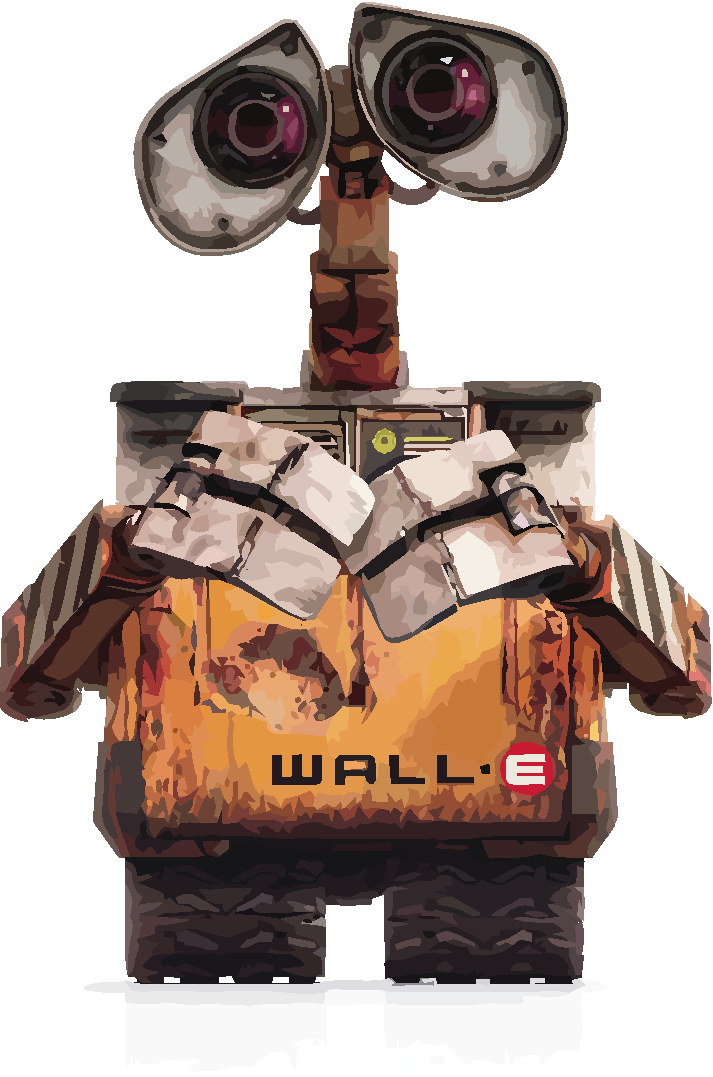
\includegraphics[width=\textwidth]{WallE}
    \caption{Wall-E}
    \label{fig:WallE}
  \end{subfigure}             
  \begin{subfigure}[b]{0.3\textwidth}
    
\includegraphics[width=\textwidth]{minion}
    \caption{Minions}
    \label{fig:Minnion}
  \end{subfigure}
  \caption{Best Animations}
  \label{fig:animations}
\end{figure}


\end{landscape}



\section{Διαμόρφωση Πινάκων}

Το παρόν κεφάλαιο έχει διαμορφωθεί με βάση το ``Publication quality tables in \LaTeX*''
 από τον Simon Fear. Αφήνω επομένως τις οδηγίες όπως ειναι στο αυθεντικό κείμενο.

The layout of a table has been established over centuries of experience and 
should only be altered in extraordinary circumstances. 

When formatting a table, remember two simple guidelines at all times:

\begin{enumerate}
  \item Never, ever use vertical rules (lines).
  \item Never use double rules.
\end{enumerate}

These guidelines may seem extreme but I have
never found a good argument in favour of breaking them. For
example, if you feel that the information in the left half of
a table is so different from that on the right that it needs
to be separated by a vertical line, then you should use two
tables instead. Not everyone follows the second guideline:

There are three further guidelines worth mentioning here as they
are generally not known outside the circle of professional
typesetters and subeditors:

\begin{enumerate}\setcounter{enumi}{2}
  \item Put the units in the column heading (not in the body of
          the table).
  \item Always precede a decimal point by a digit; thus 0.1
      {\em not} just .1.
  \item Do not use `ditto' signs or any other such convention to
      repeat a previous value. In many circumstances a blank
      will serve just as well. If it won't, then repeat the value.
\end{enumerate}

A frequently seen mistake is to use `\textbackslash begin\{center\}' \dots `\textbackslash end\{center\}' inside a figure or table environment. This center environment can cause additional vertical space. If you want to avoid that just use `\textbackslash centering'


\begin{table}
\bicaption{Ένας κακά διαμορφωμένος πίνακας}{A badly formatted table}
\centering
\label{table:bad_table}
\begin{tabular}{|l|c|c|c|c|}
\hline 
& \multicolumn{2}{c}{Species I} & \multicolumn{2}{c|}{Species II} \\ 
\hline
Dental measurement  & mean & SD  & mean & SD  \\ \hline 
\hline
I1MD & 6.23 & 0.91 & 5.2  & 0.7  \\
\hline 
I1LL & 7.48 & 0.56 & 8.7  & 0.71 \\
\hline 
I2MD & 3.99 & 0.63 & 4.22 & 0.54 \\
\hline 
I2LL & 6.81 & 0.02 & 6.66 & 0.01 \\
\hline 
CMD & 13.47 & 0.09 & 10.55 & 0.05 \\
\hline 
CBL & 11.88 & 0.05 & 13.11 & 0.04\\ 
\hline 
\end{tabular}
\end{table}

\begin{table}
\bicaption{Ένας όμορφα διαμορφωμένος πίνακας}{A nice looking table}
\centering
\label{table:nice_table}
\begin{tabular}{l c c c c}
\hline 
\multirow{2}{*}{Dental measurement} & \multicolumn{2}{c}{Species I} & \multicolumn{2}{c}{Species II} \\ 
\cline{2-5}
  & mean & SD  & mean & SD  \\ 
\hline
I1MD & 6.23 & 0.91 & 5.2  & 0.7  \\

I1LL & 7.48 & 0.56 & 8.7  & 0.71 \\

I2MD & 3.99 & 0.63 & 4.22 & 0.54 \\

I2LL & 6.81 & 0.02 & 6.66 & 0.01 \\

CMD & 13.47 & 0.09 & 10.55 & 0.05 \\

CBL & 11.88 & 0.05 & 13.11 & 0.04\\ 
\hline 
\end{tabular}
\end{table}


\begin{table}
\bicaption{Ο πιο σωστά διαμορφωμένος πίνακας}{Even better looking table using booktabs}
\centering
\label{table:good_table}
\begin{tabular}{l c c c c}
\toprule
\multirow{2}{*}{Dental measurement} & \multicolumn{2}{c}{Species I} & \multicolumn{2}{c}{Species II} \\ 
\cmidrule{2-5}
  & mean & SD  & mean & SD  \\ 
\midrule
I1MD & 6.23 & 0.91 & 5.2  & 0.7  \\

I1LL & 7.48 & 0.56 & 8.7  & 0.71 \\

I2MD & 3.99 & 0.63 & 4.22 & 0.54 \\

I2LL & 6.81 & 0.02 & 6.66 & 0.01 \\

CMD & 13.47 & 0.09 & 10.55 & 0.05 \\

CBL & 11.88 & 0.05 & 13.11 & 0.04\\ 
\bottomrule
\end{tabular}
\end{table}



%\include{Chapter4/chapter4}
%\include{Chapter5/chapter5}
%\include{Chapter6/chapter6}
%\include{Chapter7/chapter7}
%\include{Chapter8/chapter8}

% ********************************** Back Matter *******************************
% Backmatter should be commented out, if you are using appendices after References
\backmatter

% ********************************** Bibliography ******************************
\begin{spacing}{0.9}

% To use the conventional natbib style referencing
% Bibliography style previews: http://nodonn.tipido.net/bibstyle.php
% Reference styles: http://sites.stat.psu.edu/~surajit/present/bib.htm

\bibliographystyle{apalike}
%\bibliographystyle{unsrt} % Use for unsorted references  
% \bibliographystyle{plainnat} % use this to have URLs listed in References
\cleardoublepage
\bibliography{References/references}%triangleref} % Path to your References.bib file

% If you would like to use BibLaTeX for your references, pass `custombib' as
% an option in the document class. The location of 'reference.bib' should be
% specified in the preamble.tex file in the custombib section.
% Comment out the lines related to natbib above and uncomment the following line.

% \bibliography[heading=bibintoc, title={References}]

\end{spacing}

% ********************************** Appendices ********************************

\begin{appendices} % Using appendices environment for more functunality

\include{Appendix1/appendix1}
%!TEX root = ../thesis.tex
% ******************************* Thesis Appendix B ********************************

\chapter{Installing the NTUA class file}

\LaTeX.cls files can be accessed system-wide when they are placed in the
<texmf>/tex/latex directory, where <texmf> is the root directory of the user’s \TeX installation. On systems that have a local texmf tree (<texmflocal>), which
may be named ``texmf-local'' or ``localtexmf'', it may be advisable to install packages in <texmflocal>, rather than <texmf> as the contents of the former, unlike that of the latter, are preserved after the \LaTeX system is reinstalled and/or upgraded.

It is recommended that the user create a subdirectory <texmf>/tex/latex/NTUA for all NTUA related \LaTeX class and package files. On some \LaTeX systems, the directory look-up tables will need to be refreshed after making additions or deletions to the system files. For \TeX Live systems this is accomplished via executing ``texhash'' as root. MIK\TeX users can run ``initexmf -u'' to accomplish the same thing.

Users not willing or able to install the files system-wide can install them in their personal directories, but will then have to provide the path (full or relative) in addition to the filename when referring to them in \LaTeX.


\end{appendices}
	
% *************************************** Index ********************************
% \printthesisindex % If index is present

% ********************************** Print your CV *****************************
% \include{CV/cv-prof-en}
%\cleardoublepage
%% %--------------------BEGIN DOCUMENT----------------------
\begin{cvlast}
\chapter{Βιογραφικό Σημείωμα} 
% 

\textcolor{red}{Προτείνεται στο τέλος της διατριβής να προστείθεται ένα σύντομο βιογραφικό σημείωμα. Περισσότερα cv-template \href{https://github.com/demanasta/cv_tex_templates}{https://github.com/demanasta/cv\_tex\_templates} }
%--------------------SECTIONS-----------------------------------
%Section: Personal Data
\section*{Προσωπικά Στοιχεία}
\vskip -.3cm \hrule \vskip .5cm

\begin{tabular}{r p{14cm}}
    \textsc{Ονομα:} & \textbf{Δημήτριος} \\
    \textsc{Επίθετο:} & \textbf{Αναστασίου} \\
    \textsc{Πατρώνυμο:} & Γεώργιος \\ 
    \textsc{Τόπος | Ημ. γέννησης:} & Ιωάννινα  | 09 Ιουλίου 1985 \\
\multicolumn{2}{l}{\textbf{Πληροφορίες επικοινωνίας}} \\
    \textsc{Διεύθυνση:}   & ................ \\
    \textsc{Τηλέφωνο:}     & ................. \\
    \textsc{email:}    & \href{mailto:dganastasiou@gmail.com}{dganastasiou@gmail.com}\\
    \textsc{LinkedIn:}  & \href{https://www.linkedin.com/in/demitrisanastasiou/}{https://www.linkedin.com/in/demitrisanastasiou/}\\
%     Αποθετήριο:& \href{https://github.com/demanasta}{DemAnasta[at]GitHub}\\

\end{tabular}

%section*: Education
\section*{Εκπαίδευση}
\vskip -.3cm \hrule \vskip .5cm

\begin{tabular}{r p{11.5cm}}
 \textsc{}2010-2017 &\textbf{Υποψήφιος Διδάκτορας στη Σχολή Αγρ. Τοπογράφων Μηχανικών ΕΜΠ}\\
& Πεδίο: Μελέτη Τεκτονικών Μετατοπίσεων με Χρήση Επίγειων και Δορυφορικών Γεωδαιτικών Δεδομένων'' \\
& \small Επιβλέπων: Καθ. Δημήτριος \textsc{Παραδείσης}\\
% \textsc{Ιούνιος} 2010 & \textbf{IAG School on Reference Frames}\\
%& \textit{International Association of Geodesy (IAG), Aegean University}\\
%& \textit{Mytilene, Lesvos, Greece June 7-12, 2010}\\
2003-2009&\textbf{Σχολή Αγρ. και Τοπογράφων Μηχανικών ΕΜΠ}\\
& Διπλωματική εργασία: \textit{"Μελέτη των τεκτονικών μετατοπίσεων στο Ιόνιο πέλαγος με ανάλυση χρονοσειρών GPS"}\\
%2003 & Απόφοιτος 1ου Ενιαίου Λυκείου Ιωαννίνων
\end{tabular}


\section*{\centering Κατάλογος Δημοσιεύσεων}

%Section: Publications
\subsection*{Άρθρα σε Επιστημονικά Περιοδικά}
\vskip -.3cm \hrule \vskip .5cm
\begin{enumerate}
\begin{otherlanguage}{english}
\item Ganas A., Marinou A., Anastasiou D., Paradissis D., Papazissi K., Tzavaras P. and Drakatos G. (2013). \textbf{GPS-derived estimates of crustal deformation in the central and North Ionian Sea, Greece: 3-yr results from NOANET continuous network data.} \textit{Journal of Geodynamics 67, Pages 62–71A, DOI:\url{10.1016/j.jog.2012.05.010}}
\end{otherlanguage}
\end{enumerate}

\subsection*{Ανακοινώσεις σε Πρακτικά Συνεδρίων}
\vskip -.3cm \hrule \vskip .5cm
\begin{enumerate}
\begin{otherlanguage}{english}
\item Anastasiou D., Gaifilia D., Katsadourou A., Kolivaki E., Papanikolaou X, Gianniou M., Vergos G. and Pagounis V. (2012). \textbf{First Validation of the Hellenic Vertical Datum as a Prerequisite for the Efficient Disaster and Resource Management: the “Elevation” Project.} \textit{FIG Commission 3 Workshop 2012 Spatial Information, Informal Development, Property and Housing Athens, Greece, 10-14 December.}
\end{otherlanguage}
\end{enumerate}

\subsection*{Ανακοινώσεις σε Συνέδρια}
\vskip -.3cm \hrule \vskip .5cm
\begin{enumerate}
\begin{otherlanguage}{english}
\item Anastasiou D., Papanikolaou X., Marinou A., Zacharis Z., Alatza S., Paradissis D. (2015). \textbf{GNSS processing at DSO: recent activity and current status} \textit{EUREF Analysis Center Workshop 2015, Astronomical Institute, University of Bern, Switzerland. 14-15 October.}
\item Papanikolaou X., Anastasiou D., Zacharis V., Marinou A., Tita E., Paradissis D. (2015). \textbf{Planning DSO Contribution to EUREF Densification} \textit{EUREF Analysis Center Workshop 2015, Astronomical Institute, University of Bern, Switzerland. 14-15 October.}
\item Anastasiou D., Chouliaras G., Papanikolaou X., Marinou A., Zacharis V., Galanis J., Drakatos G., Paradissis D. (2015) \textbf{Geodetic and seismological analysis of the January 26, 2014 Cephalonia Island earthquake sequence.}  \textit{26th General Assembly of the IUGG,Prague, Czech Republic, 22/6 - 2/7.}
\end{otherlanguage}
\end{enumerate}

\subsection*{Εκπαιδευτικές Σημειώσεις}
\vskip -.3cm \hrule \vskip .5cm

\begin{enumerate}
\item Αναστασίου Δ., Παανικολάου Ξ., Μαρίνου Α., Παραδείσης Δ. (2014). \textbf{Εισαγωγικές σημειώσεις στο Παγκόσμιο Σύστημα Εντοπισμού, Global Posιtioning System (GPS)} \textit{Εκπαιδευτικό Σεμινάριο "Εισαγωγή στη Γεωπληροφορική", Χαροκόπειο Πανεπιστήμιο 28/6-9/7/2014}
\end{enumerate}


%
%\vfill
%% \hfill \textit{Last update: \today}
%
%\hfill \textit{Compiled via \LaTeX}

\end{cvlast}


% ********************************** end of document ***************************

\end{document}